%!TEX root = ../thesis.tex

\thispagestyle{myheadings}

\chapter{Straw measurement angular correction}
\label{app:angularcorrection}

Copied from track fitting doc - needs to be checked and updated - check language too


The tracker straws don't measure U and V coordinates directly, but instead measure the DCA radii deriving from measured hit times. In order to utilize the minimization procedure described in \secref{sec:TrackFittingAlgorithm} on measured track parameters these radii must first be converted to U and V parameters, and similarly for the U and V errors. These conversion corrections will be dependent on the angle of the track, so it's imporant to note that during each successive iteration of the track fitting, the ``measured'' parameters are adjusted by the latest ``predicted'' momenta. It was found that for the error correction, a simple straight line correction was sufficient for ideal results, while for the position correction, it was found that a constant field correction for curved tracks was sufficient \cite{something} (maybe a docdb I have somewhere).

To calculate these corrections, first the momentum perpendicular to the straw measurement axis can be ignored since it won't affect the U or V value. The correction will depend on whether the track went to the left or right side of the wire. See Figure \ref{fig:angularCorrection} for a pictorial representation of the problem. The calculation of the right side correction follows, with the left side correction being calculated in a similar manner.

\begin{figure}[]
	\centering
	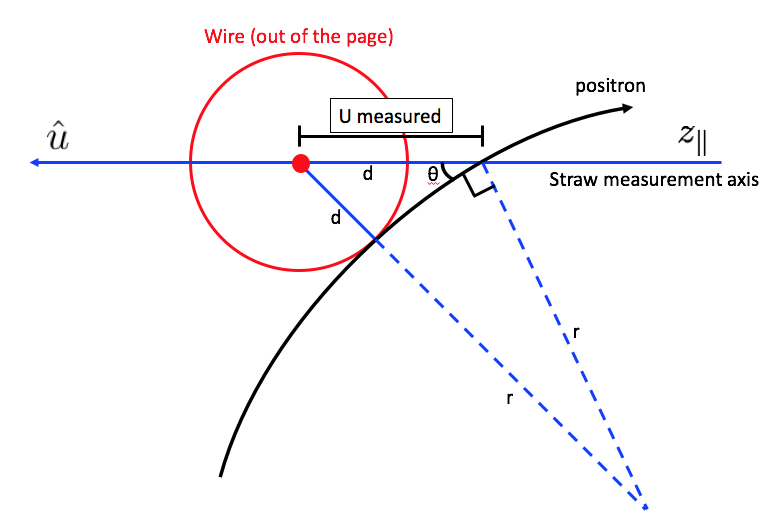
\includegraphics[width=1.0\textwidth]{angularCorrection}
	\caption{Shown here is a positron passing through a straw. The desire is to convert the measured parameter d into a U or V position, which can be done by approximating the particle trajectory as a circle in a constant magnetic field over the course of the straw and using trigonometry. Sizes and angles are exaggerated. \textbf{Might want to clean up this picture at some point.}}
	\label{fig:angularCorrection}
\end{figure}

To solve for the measured U (or V) value, we can use the equation:
\begin{align}
	(r+d)^{2} = r^{2}+u^{2}-2ru\cos(90+\theta),
\end{align}
where the 90 degrees is approximate for large curvature of tracks. The angle $\theta$ can be determined from 
\begin{align}
	\hat{z_{\parallel}} \cdot \hat{p_{\parallel}} = \cos{\theta}, \hspace{.1cm} \theta = \cos^{-1}{\frac{p_{\parallel}}{p}}, 
\end{align}
where $p_{\parallel}$ is the positron momentum parallel to the $z_{\parallel}$ axis at the wire plane and can be determined within the code. (The $z_{\parallel}$ axis simply stands for the axis perpendicular to the straw and parallel to the U measurement axis, but opposite in direction. At the end this calculated U value will simply be added or subtracted to the wire center U position depending on which side of the wire the positron travelled.) Using some trig identities and solving for u gives
\begin{align}
	u = -r\sqrt{1-(\frac{p_{\parallel}}{p})^{2}} + \sqrt{d^{2} + 2dr + r^{2}(1-(\frac{p_{\parallel}}{p})^{2})},
\end{align}
for the right side correction, and 
\begin{align}
	u = +r\sqrt{1-(\frac{p_{\parallel}}{p})^{2}} - \sqrt{d^{2} + 2dr + r^{2}(1-(\frac{p_{\parallel}}{p})^{2})},
\end{align}
for the left side correction. (Corrections to v are identical.) The radius of the particle circle can be calculated from the circular momentum and magnetic field at the predicted hit position. The straightline correction is done simply using the Pythagorean theorem in a simpler manner, with the correction to the errors then being
\begin{align}
	\sigma_{uv}' = \frac{\sigma_{uv}}{\sqrt{1-(\frac{p_{\parallel}}{p})^{2}}}.
\end{align}
